% !TeX spellcheck = en_US
\documentclass[letterpaper,12pt,twoside]{report}
\usepackage{fancyhdr}
\usepackage{fullpage}
\usepackage{tikz}
\usepackage{amsmath}

\begin{document}
	\pagestyle{fancy}
	\fancyhf{}
	\fancyhead[L]{Day 28}
	\fancyhead[R]{\textit{The Calendar Project}}
	\fancyfoot[L]{Citations Involved: none}
	
	% Problem
	\paragraph{Problem}
	\begin{quote}
		\textsf{What is an equation of the line (in y-intercept form) tangent to the graph of $x^2+y^2=25$ at the point $(3,4)$?}
	\end{quote}
	
	% Graphics
	\begin{center}
		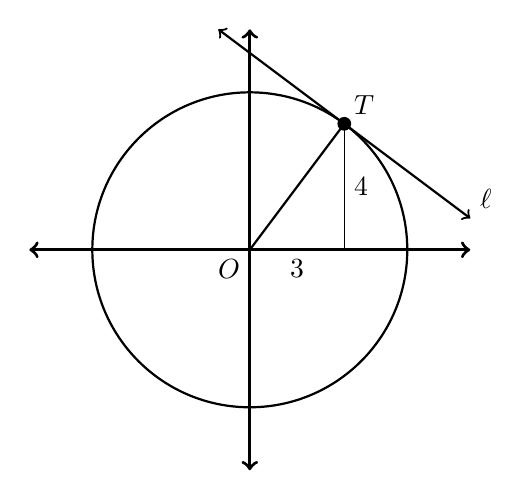
\begin{tikzpicture}[scale=0.4]
		\draw[<->,very thick] (0,7) -- (0,-7);
		\draw[<->, very thick] (-7,0) -- (7,0);
		\draw[thick] (0,0) circle [radius=5];
		\node[below left] at (0,0) {$O$};
		
		\draw[fill] (3,4) circle [radius=0.2];
		\draw (3,4) -- (3,0);
		\node[right] at (3,2) {4};
		\node[below] at (1.5,0) {3};
		\draw[thick] (0,0) -- (3,4);
		
		\draw[<->,thick] (-1,7) -- (7,1);
		\node[above right] at (7,1) {$\ell$};
		\node[above right] at (3,4) {$T$};
		\end{tikzpicture}
	\end{center}
	
	% Reasoning
	\paragraph{Reasoning}
	\begin{quotation}
		
		The given equation to which the line is tangent, $x^2+y^2=25$, applies to the form of an equation for a circle ($(x-h)^2+(y-k)^2=r^2$) (2); as such, its graph is a circle. The equation is expanded to $(x-0)^2+(y-0)^2=25=5^2$ to further fit the specified form; as such, $h=0$, $k=0$, and $r=5$, meaning that the circle's center is at $(0,0)$ and that the circle's radius is $\sqrt{25}=5$. Name the circle $O$, the tangent line $\ell$, and the point of tangency $T(3,4)$.
		
		Draw $\overline{OT}$. Since it is a radius of circle $O$ drawn to the point of tangency, it is perpendicular to $\ell$ (1). Using the slope formula, the slope of $\overline{OT}$ is determined as $\frac{y_2-y_1}{x_2-x_1}=\frac{4-0}{3-0}=\frac{4}{3}$. Since $\ell$ is perpendicular to the segment with this slope, the slope of $\ell$ is the negative reciprocal of $\frac{4}{3}$, which is $-\frac{3}{4}$.
		
		With the coordinates of $T$ and $\ell$'s slope known, the equation of $\ell$ can be expressed in point slope form: $y-4=-\frac{3}{4}(x-3)$. This is then converted to y-intercept form: $y-4=-\frac{3}{4}x-(-\frac{3}{4} \cdot 3)=-\frac{3}{4}x+\frac{9}{4} \Rightarrow y=-\frac{3}{4}x+\frac{9}{4}+4=\boxed{y=-\frac{3}{4}x+\frac{25}{4}}$.
		
	\end{quotation}
	
	\paragraph{External References}
	
	\begin{enumerate}
		\item Textbook Ch. 11, Pg. 748: Line tangent to circle $\rightarrow$ line perpendicular to radius drawn to point of tangency
		\item Textbook Ch. 11, Pg. 799: Equation of a Circle
	\end{enumerate}
	
\end{document}